\begingroup
\definecolor{probfill}{HTML}{F8FAFC}
\definecolor{probborder}{HTML}{475569}
\definecolor{probtext}{HTML}{1E293B}
\definecolor{probaccent}{HTML}{984A35}
\definecolor{probgap}{HTML}{FCF8F6}
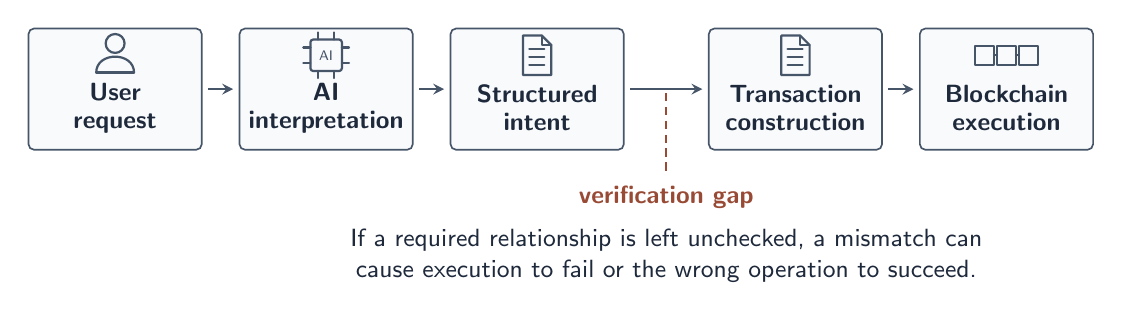
\begin{tikzpicture}[
    >=stealth,
    font=\sffamily\fontsize{10}{12}\selectfont,
    box/.style={draw=probborder,fill=probfill,text=probtext,
      rounded corners=2pt,line width=0.6pt,align=center,
      inner xsep=7pt,inner ysep=8pt},
    flow/.style={->,draw=probborder,line width=0.75pt,
      shorten <=2pt,shorten >=2pt},
    icon/.style={draw=probborder,line width=0.8pt,line cap=round,
      line join=round},
    pics/person/.style={code={
      \draw[icon] (0,0.15) circle (0.12);
      \draw[icon] (-0.24,-0.22) .. controls (-0.24,0.05)
        and (0.24,0.05) .. (0.24,-0.22);
      \draw[icon] (-0.24,-0.22)--(0.24,-0.22);
    }},
    pics/chip/.style={code={
      \draw[icon,rounded corners=1pt] (-0.2,-0.2) rectangle (0.2,0.2);
      \foreach \p in {-0.1,0.1}{
        \draw[icon] (\p,0.2)--(\p,0.29);
        \draw[icon] (\p,-0.2)--(\p,-0.29);
        \draw[icon] (0.2,\p)--(0.29,\p);
        \draw[icon] (-0.2,\p)--(-0.29,\p);
      }
      \node[text=probborder,font=\sffamily\tiny] at (0,0) {AI};
    }},
    pics/document/.style={code={
      \draw[icon] (-0.18,-0.25)--(0.18,-0.25)--(0.18,0.13)
        --(0.06,0.25)--(-0.18,0.25)--cycle;
      \draw[icon] (0.06,0.25)--(0.06,0.13)--(0.18,0.13);
      \foreach \p in {-0.12,-0.02,0.08}
        \draw[icon] (-0.10,\p)--(0.09,\p);
    }},
    pics/blocks/.style={code={
      \draw[icon] (-0.4,-0.12) rectangle (-0.16,0.12);
      \draw[icon] (-0.12,-0.12) rectangle (0.12,0.12);
      \draw[icon] (0.16,-0.12) rectangle (0.4,0.12);
      \draw[icon] (-0.16,0)--(-0.12,0);
      \draw[icon] (0.12,0)--(0.16,0);
    }}
]
% Only the five stages use boxes and arrows. The note is a margin annotation.
\foreach \id/\x/\glyph/\title in {
    req/0/person/{User\\request},interp/2.68/chip/{AI\\interpretation},
    cand/5.36/document/{Structured\\intent},build/8.64/document/{Transaction\\construction},
    exec/11.32/blocks/{Blockchain\\execution}}{
    \node[box,minimum width=2.20cm,minimum height=1.54cm] (\id) at (\x,0) {};
    \pic at (\x,0.43) {\glyph};
    \node[align=center,text=probtext,font=\sffamily\bfseries\fontsize{9}{10.2}\selectfont]
        at (\x,-0.24) {\title};
}
\draw[flow] (req.east)--(interp.west);
\draw[flow] (interp.east)--(cand.west);
\draw[flow] (cand.east)--(build.west);
\draw[flow] (build.east)--(exec.west);

% Non-directional leader touches the transition, not either stage.
\draw[draw=probaccent,densely dashed,line width=0.65pt]
    (7.00,-0.05)--(7.00,-1.08);
\node[anchor=north,text=probaccent,font=\sffamily\bfseries\small]
    at (7.00,-1.11) {verification gap};
\node[anchor=north,align=center,text=probtext,font=\sffamily\small]
    at (7.00,-1.66) {If a required relationship is left unchecked, a mismatch can\\
                      cause execution to fail or the wrong operation to succeed.};
\end{tikzpicture}
\endgroup